\documentclass[12pt]{article}

% Any percent sign marks a comment to the end of the line

% Every latex document starts with a documentclass declaration like this
% The option dvips allows for graphics, 12pt is the font size, and article
%   is the style

\usepackage[pdftex]{graphicx}
\usepackage{amsfonts}
\usepackage{amsmath}
\DeclareMathOperator*{\max_bottom}{max}
\usepackage{url}
\usepackage{hyperref}

\usepackage{caption}
\usepackage{subcaption}

\usepackage{graphicx}
\usepackage{amsmath}
\usepackage{adjustbox}
\usepackage{listings}
\usepackage{amsmath}


\lstset{language=python}

\hypersetup{
    colorlinks=true,
    linkcolor=blue,
    filecolor=magenta,      
    urlcolor=cyan,
    pdftitle={Sharelatex Example},
    bookmarks=true,
    pdfpagemode=FullScreen,
}


\usepackage{graphicx}
\graphicspath{ {./images/} }

% These are additional packages for "pdflatex", graphics, and to include
% hyperlinks inside a document.

\setlength{\oddsidemargin}{0.5cm}
\setlength{\evensidemargin}{0.5cm}
\setlength{\topmargin}{-1.6cm}
\setlength{\leftmargin}{0.5cm}
\setlength{\rightmargin}{0.5cm}
\setlength{\textheight}{24.00cm} 
\setlength{\textwidth}{15.00cm}
\parindent 0pt
\parskip 5pt
\pagestyle{plain}

% These force using more of the margins that is the default style
\newcommand{\namelistlabel}[1]{\mbox{#1}\hfil}
\newenvironment{namelist}[1]{%1
\begin{list}{}
    {
        \let\makelabel\namelistlabel
        \settowidth{\labelwidth}{#1}
        \setlength{\leftmargin}{1.1\labelwidth}
    }
  }{%1
\end{list}}


\begin{document}
\title{\Huge Noise Project Report (Diary)}

\author{
  \textbf{Pavel Rastopchin}\\
	321082026 \\ pavelr@campus.technion.ac.il
  \\ \\
  \textbf{Ameen ALi}\\
  	321082026 \\ pavelr@campus.technion.ac.il
  \\ \\ 
}

\maketitle


\newpage
\section{Q1.1}
\subsection{Problem}
\[\min_x x^T M x + c^T x\]
\[s.t: Ax - b = 0\]
\[i.e: h(x)= Ax - b = 0\]
\[M \succ 0\] 
\[i.e: M^T=M\]

\subsection{Solution}
\paragraph{Writing Lagrangian}
\[L(x, \mu)=f(x) + \mu ^T h(x) = x^T M x + c^T x + \mu ^T A x - \mu ^ T b\]

\paragraph{Finding Gradient of Lagrangian}
\[dL(x, \mu)= dx^T Mx + x^T Mdx + c^T dx + \mu ^T Adx \]
\[(dx^T Mx)\ is \ a \ scalar, \ thus: (dx^T Mx) = (dx^T Mx)^T \ thus:\]
\[dL(x, \mu) = x^T M^T dx + x^T M dx + c^T dx + \mu ^T Adx \]
\[dL(x, \mu)= (x^T M^T + x^T M + c^T + \mu ^T A)dx \]
\[dL(x, \mu)= (x^T M^T + x^T M + c^T + \mu ^T A)dx \]
\[g^T = \nabla_x L^T = (x^T M^T + x^T M + c^T + \mu ^T A)\]
\[\nabla_x L = (x^T M^T + x^T M + c^T + \mu ^T A)^T\]
\[\nabla_x L = Mx + M^T x + c + A^T \mu\]
\[M \ is \ symetric, \ thus: Mx + M^T x\ thus:\]
\[\nabla_x L = 2Mx + c + A^T \mu\]
\paragraph{KKT}
\[\nabla_x L = 2Mx + c + A^T \mu = 0 \]
\paragraph{Writing x}
\[2Mx + c + A^T \mu = 0 \]
\[2Mx = - c - A^T \mu\]
\[x = - \frac{1}{2} M^{-1}c - \frac{1}{2} M^{-1}A^T \mu\]
\paragraph{Substitute x into constraint}
\[recall\  that: Ax - b = 0\ thus:\]
\[A(- \frac{1}{2} M^{-1}c - \frac{1}{2} M^{-1}A^T \mu) - b = 0 \]
\[- \frac{1}{2} AM^{-1}c - \frac{1}{2} AM^{-1}A^T \mu - b = 0 \]
\paragraph{Writing $\mu$}
\[\frac{1}{2} AM^{-1}A^T \mu = - \frac{1}{2} AM^{-1}c - b \]
\[AM^{-1}A^T \mu = - AM^{-1}c - 2b \]
\[ \mu = (AM^{-1}A^T)^{-1}(- AM^{-1}c - 2b)\]
\[ \mu = -(AM^{-1}A^T)^{-1}(AM^{-1}c + 2b)\]
\paragraph{Substitute $\mu$ into x}
\[recall\  that: x = - \frac{1}{2} M^{-1}c - \frac{1}{2} M^{-1}A^T \mu \ \ thus:\]
\[x = - \frac{1}{2} M^{-1}c - \frac{1}{2} M^{-1}A^T (-(AM^{-1}A^T)^{-1}(AM^{-1}c + 2b))\]
\paragraph{Final answer}
\[x = - \frac{1}{2} M^{-1}c + \frac{1}{2} M^{-1}A^T (AM^{-1}A^T)^{-1}(AM^{-1}c + 2b)\]

\newpage
\section{Task 1}
\section{Q1.2.1}
\subsection{Problem}
\[min_x ||x-c||_2 ^2 = min_x (x-c)^T (x-c) = x^T x - x^T c - c^T x + c^T c\]
\[h(x)= Ax -b = 0 \]
\subsection{Solution}
\paragraph{Lagrangian}
\[L(x,\mu)=f(x) + \mu ^T h(x) = x^T x - x^T c - c^T x + c^T c + \mu ^T Ax - \mu ^T b\]
\[dL = dx^T x + x^T dx - dx^T c - c^T dx + \mu ^T Adx \]
\[those \ are \ scalars: dx^T x \ \ and \ \ dx^T c \ \ thus: \]
\[dx^T x = x^T dx \ , \ dx^T c = c^T dx \ thus: \]
\[dL = x^T dx + x^T dx - c^T dx - c^T dx + \mu ^T Adx \]
\[dL = 2x^T dx - 2c^T dx + \mu ^T Adx \]
\[dL = (2x^T - 2c^T + \mu ^T A)dx \]
\[\nabla_x L = (2x^T - 2c^T + \mu ^T A)^T = 0 \]
\[\nabla_x L = 2x - 2c + A^T \mu = 0 \]
\[x= c - \frac{1}{2} A^T \mu \]
\paragraph{Substitute x into constraint}
\[A(c- \frac{1}{2} A^T \mu) = b\]
\[Ac - \frac{1}{2} AAT^ \mu = b\]
\[AA^T \mu = 2Ac - 2b\]
\[\mu = 2 (AA^T)^{-1} (Ac - b)\]
\paragraph{Substitute $\mu$ into x}
\[x = c - \frac{1}{2} A^T ( 2 ( AA^T )^{-1} ( Ac - b ) ) \] 
\[x = c -  A^T (AA^T)^{-1} (Ac - b)\]  

\newpage
\section{Q1.2.2}
\subsection{Problem}
\[min_x x^T A x + b^T x = min_x x_1 ^2 + 2 x_1 x_2 + 2 x_2 ^2 + x_1 - x_2 + x_3 \]
\[h(x)= x_1 + x_2 + x_3 - 1 = 0\]
\[g(x)= x_3 - 1 \leq 0 \]
\subsection{Is the problem is convex?}
The problem is convex if objective function is convex and all constraints are convex. If matrix $A$ is positive definite or positive semi-definite, then the objective is convex. Constraints are liner, so they are convex. Let's eigenvalues of $A$:

\[|A- \lambda I | = (1- \lambda)(2 -\lambda)(-\lambda)+ \lambda = 0 \]
\[\lambda (- \lambda ^2 + 3 \lambda - 1  = 0\]
\[\lambda_{1,2} = \frac{+3 \pm \sqrt{5}}{2} > 0 \ , \ \lambda_3 = 0 \ \ thus: \]
\[A \succeq 0 \longrightarrow the \ problem \ is \ convex \]

\subsection{Dual problem}
\paragraph{Minimization of L in x}
\[L(x, \lambda, \mu) = x_1 ^2 + 2 x_1 x_2 + 2 x_2 ^2 + x_1 - x_2 + x_3 + \lambda (x_3 - 1) + \mu (x_1 + x_2 + x_3 - 1)\]
\[\frac{\delta L}{\delta x_1} = 2x_1 + 2x_2 + 1 + \mu = 0 \]
\[\frac{\delta L}{\delta x_2} = 2x_1 + 4x_2 - 1 + \mu = 0 \]
\[\frac{\delta L}{\delta x_3} = 1 + \lambda + \mu = 0\]
Solving equations system and denoting $\mu = -1 -\lambda$ we get:
\[x_1 = \frac{1}{2} \lambda -1 \ , \ x_2 =1 \ , \ x_3 = 1 - \frac{1}{2} \lambda\]
\paragraph{Substitute x into L to get the dual problem}
\[\eta(\lambda , \mu) = \min_x L(x, \lambda, \mu) = L(x^*, \lambda, \mu) = \]
\[= (\frac{1}{2} \lambda - 1)^2 +2(\frac{1}{2} \lambda - 1)+2+(\frac{1}{2} \lambda - 1)-1+(1 - \frac{1}{2} \lambda)+ \lambda(1 - \frac{1}{2} - 1) + \mu(\frac{1}{2} \lambda - 1 + 1 + 1 - \frac{1}{2} \lambda - 1) = \]
\[= - \frac{1}{4} \lambda ^2 \longrightarrow \eta(\lambda , \mu) = - \frac{1}{4} \lambda ^2\]
\paragraph{Maximization of the dual problem}
Instead of maximizing, we can minimize negative dual problem.
\[ \min_{\lambda \geq 0} -\eta(\lambda , \mu) = \min_{\lambda \geq 0} \frac{1}{4} \lambda ^2\]
\[\frac{\delta \eta}{\delta \lambda} = \frac{1}{2} \lambda = 0 \longrightarrow \lambda=0 \]
\[recall: \ \mu = -1 - \lambda \longrightarrow \mu = -1\]
\[x_1 = \frac{1}{2} \lambda -1 = 0 \ , \ x_2 =1 \ , \ x_3 = 1 - \frac{1}{2} \lambda\ = 1\]

\newpage
\section{Q1.3}
\subsection{Problem}
\[min_x c^T x\]
\[s.t. \ g_1 (x) = Ax-b \leq 0 \]
\[s.t. \ g_2 (x) = -x \leq 0 \]

\paragraph{Minimization of L in x}
\[L(x,\lambda_1, \lambda_2) = c^T x + \lambda_1 ^T (Ax-b) + \lambda_2 ^T (-x)\]
\[L(x,\lambda_1, \lambda_2) = c^T x + \lambda_1 ^T Ax - \lambda_1 ^T b - \lambda_2 ^T x\]
\[dL = c^T dx + \lambda_1 ^T A dx - \lambda_2 ^ T dx \]
\[dL = (c^T + \lambda_1 ^T A - \lambda_2 ^T)dx \]
\[\nabla_x L = (c^T + \lambda_1 ^T A - \lambda_2 ^T)^T = c+A^T \lambda_1 - \lambda_2 =0\]
\[c=\lambda_2 - A^T \lambda_1\]
\paragraph{Substitute c into L to get the dual function}
\[L(x,\lambda_1, \lambda_2) = (\lambda_2 - A^T \lambda_1)^T x + \lambda_1 ^T (Ax-b) + \lambda_2 ^T (-x) = -\lambda_1 ^T b\]
  \[
    \eta(\lambda_1 , \lambda_2) =\left\{
                \begin{array}{ll}
                  -\lambda_1 ^T b \ \ ; \ c=\lambda_2 - A^T \lambda_1 \\
                  - \inf \ \ ; \ otherwise
                \end{array}
              \right.
  \]
\paragraph{Dual problem}
Instead of maximizing we can minimize negative dual function. 
\[\min_{\lambda \geq 0} \lambda_1 ^T b\]
\[s.t. \ c=\lambda_2 - A^T \lambda_1\]


\newpage
\section{Task 2}
\subsection{Problem}
\[\min_x 2(x_1-5)^2+(x_2-1)^2\]
\[s.t \ \ x_2 \leq 1- \frac{x_1}{2} \longrightarrow g_1(x)=x_2-1
+\frac{x_1}{2} \leq 0 \]
\[x_2 \geq x_1 \longrightarrow g_2(x)=x_1-x_2 \leq 0 \]
\[x_2 \geq - x_1 \longrightarrow g_3(x)=-x_1-x_2 \leq 0 \]

\subsection{Feasible area}
\begin{figure}[h]
\centering
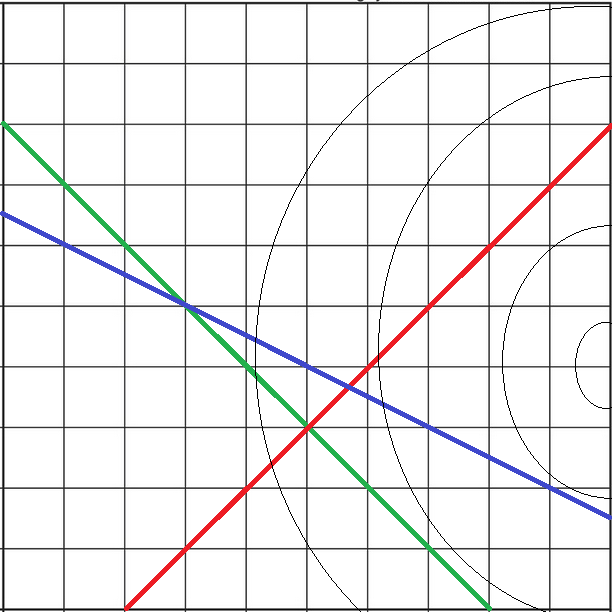
\includegraphics[width=0.7\textwidth]{pics/feas}
\end{figure}
Active constrains are red and blue lines. which is $g_1$ and $g_2$, thus $\lambda_3 = 0$.

\subsection{Optimal solution at the intersection of the active constraints}
\[x_1=x_2 , x_2=1-\frac{x_1}{2} \longrightarrow x_2 = \frac{2}{3}, x_1=\frac{2}{3} \]
\[f(x_1,x_2) = 37 \frac{2}{3} \]

\subsection{Calculate the Lagrange multipliers}
\[\L=2(x_1-5)^2+(x_2-1)^2 +\lambda_1(x_2-1
+\frac{x_1}{2}) +\lambda_2(x_1-x_2) \]
\[\frac{\delta L}{\delta x_1} = 4 x_1 -20 + \frac{1}{2} \lambda_1 + \lambda_2 = 0 \longrightarrow x_1^* = \frac{20-\frac{1}{2}\lambda_1-\lambda_2}{4} \]
\[\frac{\delta L}{\delta x_2} = 2x_2-2+\lambda_1-\lambda_2=0 \longrightarrow x_2^*=\frac{2-\lambda_1+\lambda_2}{2} \]
\[by \ \ KKT: \lambda_i g_i(x^*)=0 \]

\[
\left\{
\begin{array}{ll}
-9\lambda_1+6\lambda_2+40=0 \\
3\lambda_1-6\lambda_2+32=0
\end{array}
\right.
\]

\[\lambda_1=12 \ , \ \lambda_2=11\frac{1}{3} \]

\subsection{Optimal value of objective function}
\[
\left\{
\begin{array}{ll}
x_1^* = \frac{20-\frac{1}{2}\lambda_1-\lambda_2}{4} \longrightarrow x_1^* = \frac{2}{3}\\
x_2^*=\frac{2-\lambda_1+\lambda_2}{2} \longrightarrow x_2^* = \frac{2}{3}
\end{array}
\right.
\]

\[f(x_1^*,x_2^*)=37 \frac{2}{3} \]

\subsection{Dual problem}
\[\eta(\lambda_1, \lambda_2) = 2(-\frac{1}{8}\lambda_1-\frac{1}{4}\lambda_2)^2 + (-\frac{1}{2}\lambda_1+\frac{1}{2}\lambda_2)^2 + \lambda_1 (-\frac{9}{16}\lambda_1 +\frac{3}{8}\lambda_2+\frac{5}{2})+\lambda_2 (4+\frac{3}{8}\lambda_1-\frac{3}{4}\lambda_2) \]
\[\min_{\lambda \geq 0} -\eta(\lambda_1, \lambda_2) \]

\subsection{Substitute the obtained in Q.3 Lagrange multipliers}
Is the dual optimum achieved at that point? Yes.
\[\eta(\lambda_1^*, \lambda_2^*) = 37 \frac{2}{3} \]

\newpage
\section{Code}
\subsection{Penalty method}
\subparagraph{Lagrangian} Lets look at example with only one constraint
\[L_{p\mu}(x) = f(x) + \mu_i \varphi_{p }(g_{i(x)}) + ... \]

\[\nabla_x L_{p\mu}(x) = \nabla_x f(x) + \mu_i \varphi_{p }^{'} (g_{i(x)}) \nabla_x g_{i(x)} + ... \]

\[\nabla_x^2 L_{p\mu}(x) = \nabla_x^2 f(x) +  \mu_i \varphi_{p}^{''} (g_{i(x)}) \nabla_x g_{i(x)}\nabla_x^T g_{i(x)} +  \mu_i \varphi_{p}^{'} (g_{i(x)}) \nabla_x^2 g_{i(x)} + ... = \]

\[\nabla_x^2 L_{p\mu}(x) = \nabla_x^2 f(x) +  \mu_i \varphi_{p}^{''} (g_{i(x)}) \nabla_x g_{i(x)}\nabla_x^T g_{i(x)} + 0 \]

\subparagraph{Penalty Function}
\[
    \varphi_{p}(g_{(x)}) =\left\{
                \begin{array}{ll}
                  \frac{1}{p}(\frac{p^2 g_{(x)}^2}{2} + pg_{(x)}) \ ; \ pg_{(x)} \geq -\frac{1}{2} \\
                  \frac{1}{p} [-\frac{1}{4} \log(-2pg_{(x)})-\frac{3}{8}] \ ; \ pg_{(x)} -\frac{1}{2}
                \end{array}
              \right.
\]

\[
    \varphi_{p}^{'}(g_{(x)}) =\left\{
                \begin{array}{ll}
                  (pg_{(x)}+1) \ ; \ pg_{(x)} \geq -\frac{1}{2} \\
				-\frac{1}{4pg_{(x)}}\ ; \ pg_{(x)} < -\frac{1}{2}
                \end{array}
              \right.
\]

\[
    \varphi_{p}^{''}(g_{(x)}) =\left\{
                \begin{array}{ll}
                   p \ ; \ pg_{(x)} \geq -\frac{1}{2} \\
				\frac{1}{4pg_{(x)}^2}\ ; \ pg_{(x)} < -\frac{1}{2}
                \end{array}
              \right.
\]

\end{document}
